%%%%%%%%%%%%%%%%%%%%%%%%%%%%%%%%%%%%%%%%%%%%%%%%%%%%%%%%%%%
% EPFL report package, main thesis file
% Goal: provide formatting for theses and project reports
% Author: Mathias Payer <mathias.payer@epfl.ch>
%
% This work may be distributed and/or modified under the
% conditions of the LaTeX Project Public License, either version 1.3
% of this license or (at your option) any later version.
% The latest version of this license is in
%   http://www.latex-project.org/lppl.txt
%
%%%%%%%%%%%%%%%%%%%%%%%%%%%%%%%%%%%%%%%%%%%%%%%%%%%%%%%%%%%
\documentclass[a4paper,11pt,oneside]{report}
\usepackage[BScProject,lablogo]{EPFLreport}
\usepackage{xspace}
\usepackage{amsmath}
\usepackage{amsthm}
\usepackage{graphicx}
\usepackage{subcaption}

\title{Flatpak attestation using Reproducible Builds}
\author{Zacharie Timothée Tevaearai}
\supervisor{Flavio Toffalini}
\adviser{Prof. Dr. sc. ETH Mathias Payer}

\theoremstyle{definition}
\newtheorem{definition}{Definition}[section]

\newcommand{\sysname}{flatpak-rebuilder\xspace}
\newcommand{\Sysname}{Flatpak-rebuilder\xspace}
\newcommand{\rb}{reproducible builds\xspace}
\newcommand{\fp}{flatpak\xspace}
\newcommand{\Fp}{Flatpak\xspace}
\newcommand{\fh}{flathub\xspace}
\newcommand{\fb}{flatpak-builder\xspace}
\newcommand{\fdp}{flatpak dependencies\xspace}
\newcommand{\sde}{SOURCE\_DATE\_EPOCH\xspace}
\newcommand{\ldlp}{LD\_LIBRARY\_PATH\xspace}
\newcommand{\fhbb}{flathub buildbot\xspace}
\newcommand{\dfc}{diffoscope\xspace}
\newcommand{\ot}{OSTree\xspace}


\begin{document}
\maketitle

\begin{abstract}
Software can be built from source code or distributed as pre-compiled packages.
These packages are the result of a software supply chain which can be
subject to attacks or bugs and cannot be trusted. A way to attest that a
product from such a supply chain corresponds to its original source code is
called \rb and consists in performing the exact build steps, for a certain
package, independently of the main supply chain and comparing the rebuilt
artifact with the original one. If they are bit by bit identical, then we
prove that the path between the source code and the final artifact is
legitimate. Here we look at the possibility of using reproducible builds
with \fp, a packaging technology used to ship the same binaries on multiple
Linux distributions. In particular, we focus on \fh, its main repository.
We present a tool, called \sysname, which rebuilds a package available on
\fh, by recreating a minimal environment. We then measure the amount of
non-reproducible packages, and find out that it represents 59\% of packages
on \fh. We then do further analysis to understand why they are not
reproducible and conclude that we can reach 60\% of reproducible programs
by providing extra information to recreate the environment, the key one
being the time at which the build take place.
\end{abstract}

\maketoc

%%%%%%%%%%%%%%%%%%%%%%
\chapter{Introduction}
%%%%%%%%%%%%%%%%%%%%%%


In theory, with free and open source software (FOSS) we can audit the code and
compile only software we trust. In reality most software are shipped as
pre-built binaries to end-users, through a software supply chain. In this
context how can we be sure that the resulting artifact is produced from the
original source code ? Indeed, the machine on which the software was compiled
might be compromised, a bug may occur during the process, or some maintainer
may manually add a malicious patch to the final product. There are all sorts of
reasons to not trust what is shipped to the end-users. Supply chain attacks can
be conducted on both open source and closed source software, and typically
consist in injecting malicious code into an existing product. Examples include
the SolarWinds exploit from 2020, where attackers had compromised the update
publishing infrastructure of Orion, one of SolarWinds software, and were
shipping a modified version with a malware injected~\cite{enwiki:solarwinds}.
In the FOSS world, attacks targeting package manager such as npm or RubyGem
occurred and are already studied in the
literature~\cite{10.1007/978-3-030-52683-2_2}.
Techniques exist to counter such attacks, and the one we use in this project is
called \emph{\rb}~(R-B). It is a set of practices to make sure we can,
independently of the supply chain, obtain the same package, bit by bit,
starting from the source code, by reproducing the exact same build steps. The
exact definition for a build process to be reproducible, as stated by Chris
Lamb and Stefano Zacchiroli, is as follows:

\begin{definition}[reproducible build]
\label{def:reprobuild}
``\emph{The build process of a software
product is reproducible if, after designating a
specific version of its source code and all of its
build dependencies, every build produces bit-for-
bit identical artifacts, no matter the environment
in which the build is performed.}''~\cite{DBLP:journals/corr/abs-2104-06020}
\end{definition}

If a piece of software is reproducible we can therefore attest its integrity,
by reproducing it on our side and comparing it with the one resulting from an
untrusted build process. For example, we can use it with a Linux distribution.
Here users download, through a package manager, programs which are built by the
distribution vendor. A hypothetical \rb setup, like in
\autoref{fig:reprobuild}, would go as follows: The source code is produced
upstream and is published on platform such as GitHub or GitLab. Maintainers
then build it on some infrastructure, with certain dependencies and a specific
tool chain. They sign and send the resulting artifact to the end-user. This
process, as shown before, cannot be trusted. On the other hand upstream code
can be audited and verified manually. Now, the maintainers, alongside the
build, can record and publish the necessary information to redo the build
with the same conditions. This information will include, among others, the
exact dependencies and which version of the tool chain were used. From these, a
set of trusted rebuilder will redo the build and publish
the checksum of the artifact they obtain. When the end-user download a program
from the distribution's repositories, they can compare the checksum they have
with the one given by the rebuilders and can then decide to trust or not what
they just downloaded. The exact process of deciding if the artifact is
legitimate by comparing the checksums can be automated, and computed
differently depending on the number of independent rebuilder and how much we
trust them.
Using \rb we can prove that the path between upstream and downstream is
legitimate. Since we can audit and trust the source code, this trust can
propagate to the build artifact, without the cost of auditing binaries. An
attacker would have to take over not only the supply chain, but also a certain
amount of these independent rebuilder (depending on how we compare the
checksums), reducing the feasibility of such attacks. Integrity also proves us
that no bugs or errors occurred during the build. The practicality of using \rb
to provide integrity for a software supply chain has already been shown, for
instance on Debian, where $82.5\%$ of packages on the unstable branch are
reported as reproducible as of \today~\cite{debian:repro}.

\begin{figure}[h]
    \center{
        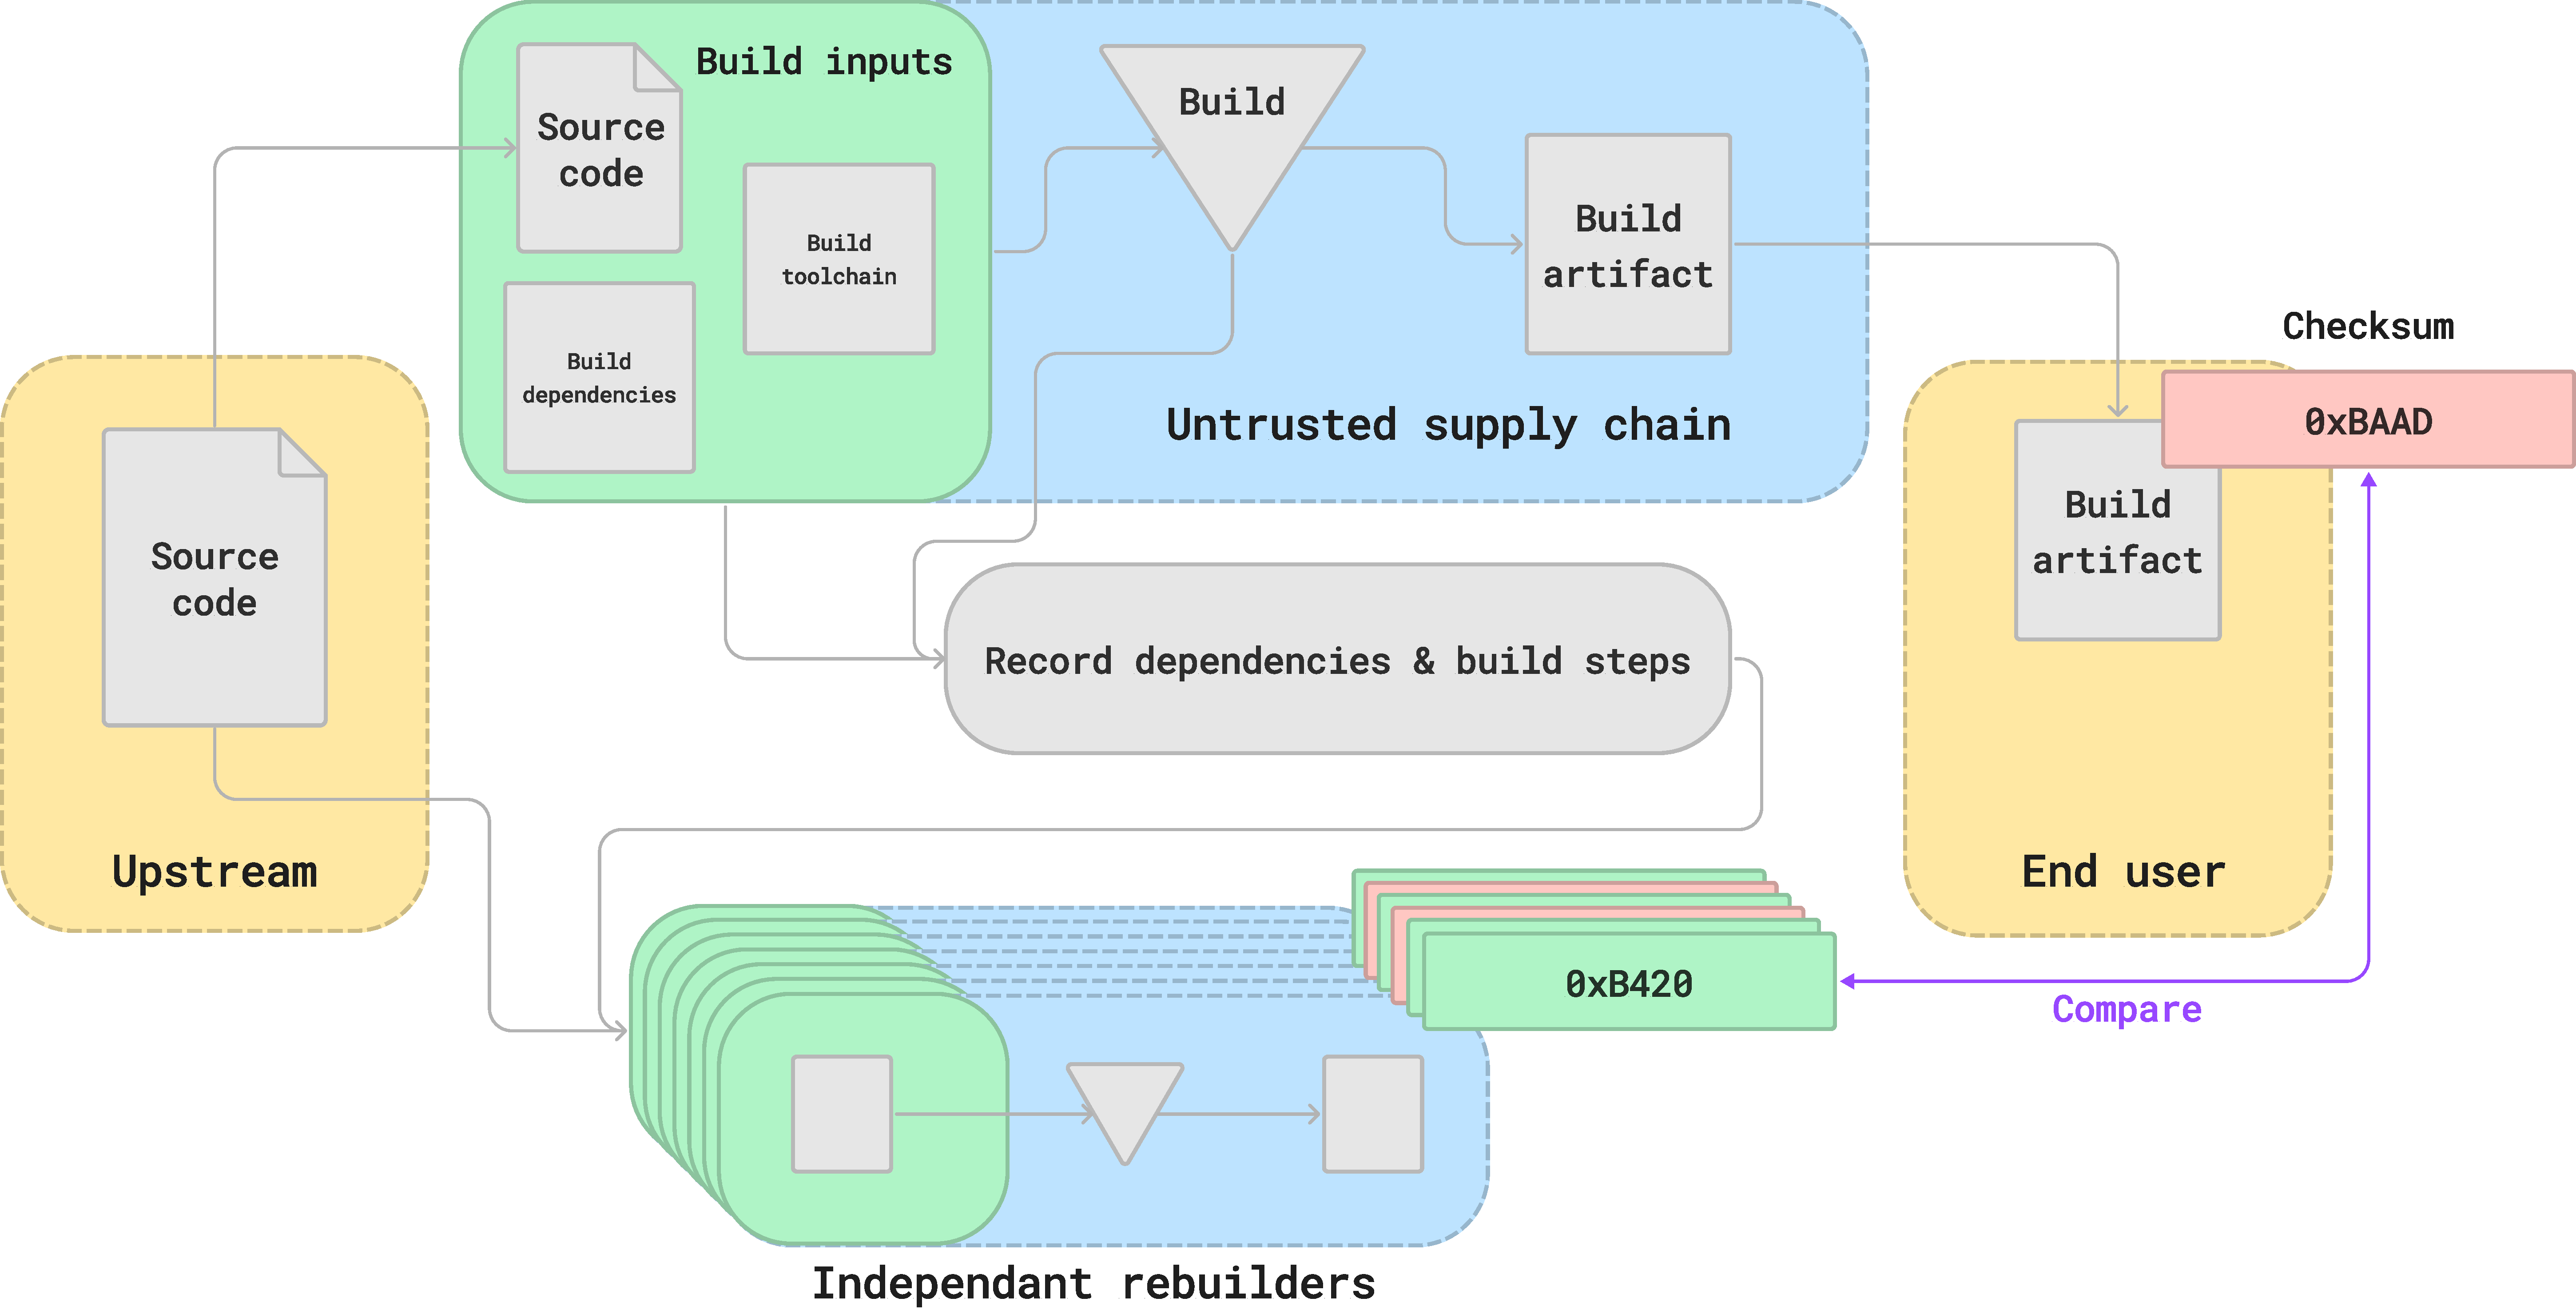
\includegraphics[width=\textwidth]{figures/Kokodayo.pdf}
    }
    \caption{A reproducible builds setup. Here the end user can compare the
    checksum of the package they download, with a set of independent
    rebuilders. Since in majority the checksums do not match, they reject the
    package. Adapted from~\cite{DBLP:journals/corr/abs-2104-06020}.}
    \label{fig:reprobuild}
\end{figure}

One software distribution system that can benefit from \rb is \emph{\fp}, and
more precisely its main repository called \emph{\fh}. \Fp is way to build,
distribute and deploy applications compatible on most Linux distributions. It
works by running them inside a container (which is referred to as a sandbox)
where they have the minimum permissions and are as much isolated as possible
from the host system. Since the build can also be performed inside the sandbox,
it is an ideal environment to use \rb. However, there are no tools to redo the
build of a \fp from \fh, and therefore there are no statistics on how many
flatpaks are reproducible. In this project, we create a tool called
\emph{\sysname}, to allow individual to redo a build of a \fp from \fh, and
attest if it produces the same artifact or not. Using \sysname we then measure
the amount of reproducible programs on \fh, and provide improvement to the \fh
build infrastructure, in order to increase this number. Since \fp works across
Linux distributions, \sysname needs to be as portable. This limits the use of
strong container technologies, such as Docker, or tools such as \verb|faketime|
to better simulate the build environment.
After rebuilding 729 programs, which is about half of \fh, we have 41\%
reproducible programs, which is much lower than what is found on Debian. This
is mainly due to the lack of certain information, such as the time at which the
build originally took place. Consequently, we propose several improvements to
\emph{\fb}, the main tool used to build \fp on \fh, which is also the one
capable of recording some missing build information. We also introduce new
notions to characterize how reproducible a program is, such that we can still
build trust in programs which are only partially reproducible.

The structure of the report is the following, \autoref{chap:bg} explains all
the concept used in the next chapters. In \autoref{chap:design} and
\autoref{chap:impl} we describe the overall functioning of \sysname. In
\autoref{chap:eval} we measure the reproducibility of \fh and provide a manual
analysis of the main causes of non-reproducibility. Finally, in
\autoref{chap:relw} we discuss and compare our approach to other similar tools,
and also compare \rb as a whole to other techniques to secure the supply chain.

\section{Motivation}
No tools exist to easily redo a build of a \fp from \fh, consequently there are
no measurement of how many flatpaks are reproducible. This implies that there
are no knowledge about issues, specific to \fp, concerning the feasibility of
\rb there. The main goal, is to have a first idea of the problems of applying
\rb to \fp and then to use that knowledge to further improve the situation. The
challenge is that since no one really tried to know if flatpaks are easily
reproducible or not, we will not have access to all the information to properly
recreate a build environment which resemble the one used to build programs on
\fh. Indeed, on Debian for instance, it is only after they started to measure
the amount of reproducible program on their repositories, that they could
improve the situation. And as a matter of fact, they started with fairly low
ratio of reproducible programs, at the beginning (roughly
60\%)~\cite{debian:repro}. We therefore expect in this project to reach a
fairly low amount of reproducible program, but also to find ways to greatly
improve it.


%%%%%%%%%%%%%%%%%%%%
\chapter{Background}
\label{chap:bg}
%%%%%%%%%%%%%%%%%%%%

To better understand this project, we should introduce a bit more \rb,
especially the most common reasons a program may not be reproducible. From
\autoref{def:reprobuild}, we conclude that a build is not reproducible when
after performing the exact same build steps, with the same build dependencies,
we reach another result. One reason it could happen is when a program depends
on more than just its build dependencies. Typical examples are build process
affected by the time or the path in which the build took place. This is what C.
Lamb refer to as \emph{uncontrolled build input}, because the build is affected
by additional inputs which are not under our control. In practice some of these
issues (such as time) can be solved if we include these as extra dependencies
to the original definition of \rb. It can be tempting to put the whole
environment as a dependency (kernel version, CPU model, etc.) but doing so will
make the rebuilding step much harder and will slow down build time, which would
not make \rb a practical solution. To mitigate the effects of
\emph{uncontrolled build input}, we rely on another definition of reproducible:
\begin{definition}[reproducible build]
\label{def:reprobuild2}
``\emph{A build is reproducible if given the same source code, build
    environment and build instructions, any party can recreate bit-by-bit
    identical copies of all specified artifacts.
The relevant attributes of the build environment, the build instructions and
    the source code as well as the expected reproducible artifacts are defined
    by the authors or distributors. The artifacts of a build are the parts of
    the build results that are the desired primary output.}''~\cite{reprobuilds:def}
\end{definition}
This definition come from the \emph{Reproducible Builds project}~(R-B project),
an organization which promotes \rb. A good example of "relevant attributes of
the build environment", are the \verb|.buildinfo| files on
Debian~\cite{debian:buildinfo}. Those are files associated to a package,
describing the environment in which the build took place. Not everything in a
\verb|.buildinfo| is necessary to perform a rebuild (for instance the kernel
versions), but certain information, such as the time or the active environment
variables are easy to manipulate and can be considered as valid additional
input for the build process. In particular, time can be controlled by
overriding the \sde environment variable. It is defined as part of the R-B
project, and can be consumed by build systems to make sure the resulting build
looks like it was done entirely at the time specified by the
variable~\cite{rb:sde}.
Other than uncontrolled build inputs, there is another class of problems
affecting the reproducibility of a program, which is \emph{build
non-determinism}. It occurs when some parts of the build are random. One
example is the serialization of frozenset items in Python, which does not
happen in a deterministic order~\cite{gh:pyc-frozenset}. Other non-determinism
issue can be for instance related to the parallelism of the build process, or
to filesystem ordering, since both do not follow a strict order. Even though
work still need to be done in order to have deterministic builds for certain
build systems, such as with Java~\cite{xiong2022towards}, the most common one
can behave deterministically.


The other main concept to introduce is \fp and \fh, more specifically how a \fp
is built and shipped on \fh. As stated before, flatpaks are deployed and built
inside a sandbox, a container mostly isolated from the host system. Extra
permissions, such as access to certain directories, access to the network and
so on, are managed in the metadata of a \fp. There are no general build process
for a \fp. As long as the build directory respect certain conventions, and the
necessary metadata are accessible at the root, it is a valid \fp. The way \fp
are shipped and deployed is through \ot. It is a library, working similarly as
git, but optimized to handle binary objects. Furthermore, it is specialized to
handle entire file system trees. \Fp uses it in the following way, the build
directory of a program is committed through \ot and can be push to a remote and
pulled by end-users. \ot is used to deploy a read-only, using hard links,
version of the \fp, which is mounted inside the sandbox (at /app). Since
flatpaks are isolated from the host, they cannot access its libraries, such as
libc. Instead, those are bundled with the \fp and therefore also mounted in the
sandbox. While this works and ensure a program built against one library will
not suddenly run against another version, this has multiple issues. First it is
not disk efficient, for instance almost every program will ship with libc.
Secondly, security critical libraries such as libssl need regular updates, and
having each \fp shipping their own copy increases the risk of having some which
are out of date. To address these issues, \fp comes with a simple shared
dependencies systems called \emph{runtimes}. A \fp will always depend on a
specific runtime (specified in its metadata), which is another \fp containing
the most common and security critical dependencies. The runtime is also mounted
in the sandbox, with the main app. Another runtime, called the \emph{SDK},
exists, it just includes additional dependencies only useful at build time, or
for debugging purposes, such as gdb and gcc. A \fp can also depend on a
\emph{base-app}, which is a \fp containing certain big build dependencies, for
certain type of applications, such as those based on Electron. Finally, a last
type of dependencies are extensions, for SDK or base-app, which are just
additional libraries or programs that can be optionally mounted. An example is
the Rust tool chain, which is available as an SDK-extension, such that only
rust programs needs to include it at build time. The build process is not
standardized, a \fp can be built using any build system available. However, a
helper tool called \fb exists and is used on \fh. It parses a description of
the build, called a manifest file, and produces the resulting \fp. The manifest
is separated in modules, where each describes how to build one dependency or
the final program, and each specifies how to fetch the necessary build
dependencies. The manifest also includes which runtime and SDK need to be used
and which permissions need to be applied to the resulting \fp. Flathub, the
main repository for \fp, is a community based project, where each application
has a GitHub repository under the \fh organization. These repositories contain
at least the manifest file to build the app using \fb. The \fhbb is a bot which
after any commit to the master branch of an application will fetch and build
the manifest file. The resulting artifact is committed using \ot and pushed to
the \fh remote.


%%%%%%%%%%%%%%%%
\chapter{Design}
\label{chap:design}
%%%%%%%%%%%%%%%%

This section describes the high-level functioning of \sysname, it is summarized
in \autoref{fig:flatpakrebuilder}.

\section{Recreating the environment}
To rebuild a program, \sysname must first make sure to gather all build
dependencies to the exact version used during the original build. There are two
types of dependencies defined in a \fb manifest file, the one which are
embedded in the final package, those are defined in the different modules of
the manifest and their version is always perfectly specified. For instance a
dependency on a git repository will come with the hash of the commit. Those
dependencies are therefore easy to gather, and it is already handled by \fb.
The other type of dependency is what we refer to as \emph{\fdp}. They are
dependencies of the form of a \fp, and are mounted in the sandbox during the
build and sometimes also when running the final app. Those dependencies include
runtimes, SDK, SDK-extensions, base-app and base-app extensions. In the case of
\fh, they will come from \fh directly, but the original manifest does not
include the exact \ot commit associated to each of them. Fortunately, \fb will
ship a modified version of the manifest in the final product, which include the
commit of the runtime, the SDK, and (if there is any) the base-app.
Unfortunately it will not include the one for SDK-extensions and base-app
extensions, but we know the \fhbb will use the latest version available at the
time of the build. However, the exact time of the build is also not specified,
it is bounded by the commit to GitHub, which is before and the \ot commit,
which happens after the build. We therefore guess which commit was used by
taking the latest available at the \ot commit time. This will introduce some
error, but we will show that it is relatively small. Another dependency we need
to pin to its exact version is \fb itself. In the case of the \fhbb, it uses
the last one available on \fh. We therefore consider it as any other \fdp, and
apply the same guessing technique.
To manipulate the time of the build, we override the \sde variable. Under the
hood, \fb overrides it with the last modification time of the manifest file,
but this information is lost when a file is committed to git or \ot . We
therefore do as before, and use the \ot commit time to override \sde, which is
another source of error.

\section{Rebuilding}
Once the environment matches roughly the one from the original build, we need
to execute the exact same steps done by the \fhbb. Since its code is
open-source, we merely follow the same code, we just ignore the verification
and exporting steps done at the end.

\section{Measuring reproducibility}
\label{sec:measure}
At the end of a rebuild we compare the checksum of the original package, with
the rebuilt one, and conclude that the build is reproducible if the two are the
same. This follows a very strict definition of reproducibility, and we
therefore introduce three more reproducibility tests. The first is the notion
of binary-reproducibility, where we compute the hash of only non human-readable
files (ELF, images, archives, etc.). The second is ELF-reproducibility, where we
only compare ELF files, and the last one is the repro-score, which is defined
as the number of non-reproducible files over the total number of files. The
reasoning behind the binary and ELF reproducibility is the following: we can
still audit and understand non-binary files, and therefore if the only sources
of non-reproducibility are in files we can easily verify manually, we can still
attest that the build is legitimate, even if it is only partially reproducible.
The idea behind the repro-score is to find a way to automatically differentiate
a program which is highly non-reproducible, from those which are mostly
reproducible, by assuming that a program with a high repro-score will be easy
to fix, and make reproducible.

\begin{figure}[h]
    \center{
        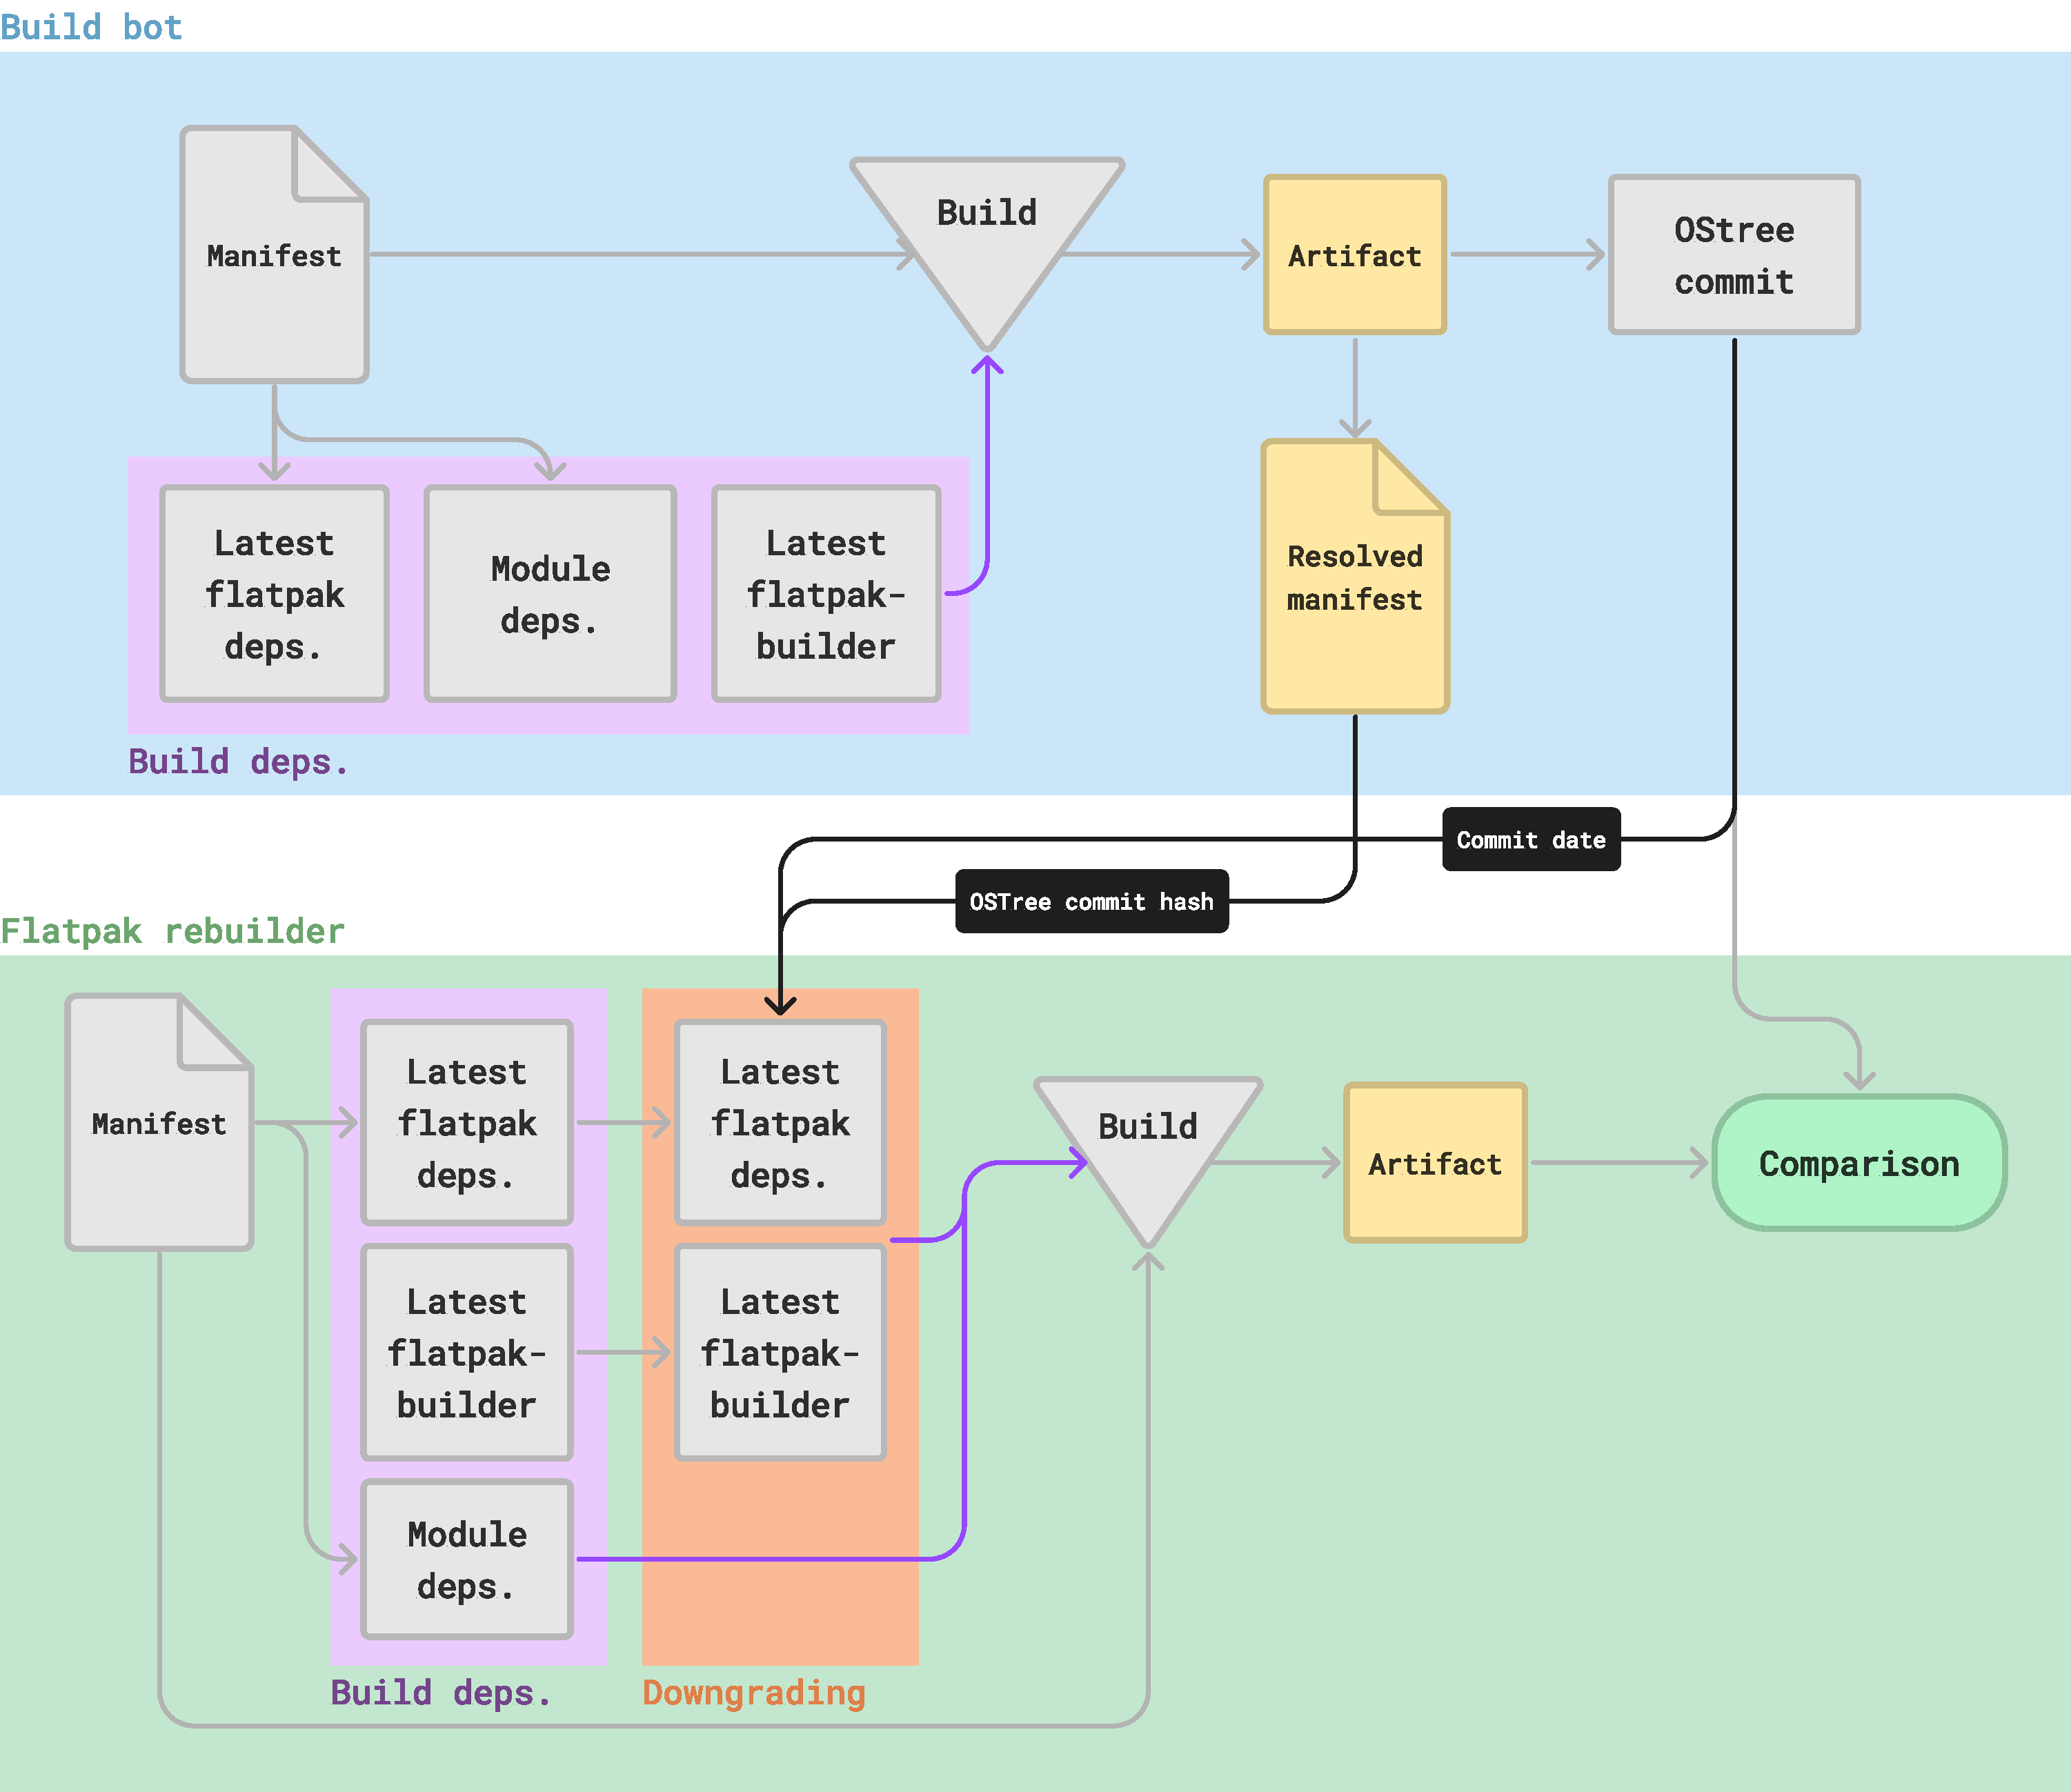
\includegraphics[width=\columnwidth]{figures/I_Droped_Saga.pdf}
    }
    \caption{High level description of \sysname.}
    \label{fig:flatpakrebuilder}
\end{figure}

%%%%%%%%%%%%%%%%%%%%%%%%
\chapter{Implementation}
\label{chap:impl}
%%%%%%%%%%%%%%%%%%%%%%%%

For simplicity, and portability, \sysname is written in python, using the poetry
package manager, both available on any platform susceptible to run \fp. Other
than python, it relies on GNU coreutils, which should also be supported on most
Linux distribution, and optionally uses two external tools, diffoscope and
strip-nondeterminism. Both are developed as part of the R-B project. Diffoscope
is used to compute the difference between two artifacts, by going deeply inside
the file tree, even doing things such as diffing recursively archives.
Strip-nondeterminism is a tool to strip certain non-necessary, but not
deterministic, bits of information, such as archives timestamps. Also, \sysname
relies on \fp, and interact with it through the CLI tool, rather than using
libflatpak. This way the code looks closer to a shell script, and matches more
the process of building manually using \fb. Also, the \fhbb does the same and
uses the CLI directly, making it easier to copy the build steps done by the
\fhbb. The overall behavior of \sysname is the following. Before rebuilding, we
first make sure the \fh remote is correctly configured, and if not, configure
it. Then we gather all \fh dependencies. To do so, we should parse the package
metadata, but instead we rely on \fb to do the work. Using the
\verb|--install-deps-from=flathub| flag, \fb figures out which dependencies are
used, and it will print them to stdout. To have the list of \fh dependencies,
we simply parse this output. As said before, \fb will take the latest
dependencies available, meaning we need to downgrade them just after. To
correctly downgrade \fh dependencies, we download the original \fp, since it
includes a modified version of the manifest file, with the exact commit of some
of these dependencies. We also need it to compare the checksum after the
rebuild. For the others, we apply the guessing technique described in
\autoref{chap:design}. Then, we pull the GitHub repository containing the
manifest file. We have to be careful to fetch the right branch, generally
master, and the right commit. Based on the \ot commit of the package, we
take the git commit which is the closest before. We also use the \ot commit
date to change the last modification time of the manifest, since \fb uses it to
internally override the \sde environment variable. From there, \sysname is
ready to rebuild. The rebuilding part occurs in three steps. First we check
that the \fh dependencies were indeed downgraded to the right version. Then we
only download the dependencies used by each module. This lets us compute a few
statistics on the amount of dependency used, and to more accurately measure the
time to build. Both are used in the analysis. Finally, we rebuild, by using the
same command run by the \fhbb. Once done, \sysname compares the checksums of
the original package against the freshly rebuilt one. On Arch Linux or Debian,
packages are distributed in an archived format, making it straightforward to
compute the checksums. Here the format is an \ot commit. To do the
comparison, we first deploy each commit, meaning we copy its content in a
concrete folder and then perform the checksums on both. During all these steps
we record different statistics, and serialize them at the end. These statistics
include, among other things, if the build succeeded or not, what dependencies
were used, what checksums were obtained. This provides an easy way to analyze
the result of a rebuild and is also a nice way to communicate it. It can be
signed and used as a replacement to the simple checksum used in
\autoref{fig:reprobuild}. The code is small (a bit more than a thousand line)
making it easy to audit.

%%%%%%%%%%%%%%%%%%%%
\chapter{Evaluation}
\label{chap:eval}
%%%%%%%%%%%%%%%%%%%%

In this part, we answer these two main project questions:
\begin{itemize}
    \item PQ1: how many applications are reproducible on \fh~?
    \item PQ2: what are the main reasons some applications are not reproducible ?
\end{itemize}
A third minor question is to know if the repro-score introduced in
\autoref{sec:measure} is a good metric. We answer it in
\autoref{sec:reprscore}. We also discuss some improvements that can be done to
the \fh supply chain in \autoref{sec:imp}

\noindent
We run several experiments, on three different machines, with the following
specifications:
\paragraph{Arch desktop}
\begin{itemize}
    \label{arch-desktop}
    \item OS: Arch Linux
    \item Kernel: 5.18.1-arch1-1
    \item CPU: AMD Ryzen 7 2700X (16)
    \item GPU: NVIDIA GeForce GTX 760
    \item Memory: 16007MiB
\end{itemize}
Running version 1.12.7 of \fp, from the Arch repository
\paragraph{Arch laptop}
\begin{itemize}
    \label{arch-laptop}
    \item OS: Arch Linux
    \item Kernel: 5.18.0-arch1-1
    \item CPU: Intel i5-5300U (4)
    \item GPU: Intel HD Graphics 5500
    \item Memory: 7828MiB
\end{itemize}
Running version 1.12.7 of \fp, from the Arch repository.
\paragraph{Fedora desktop}
\begin{itemize}
    \label{arch-desktop}
    \item OS: Fedora Linux 35 (Workstation Edition)
    \item Kernel: 5.17.5-200.fc35.x86\_64
    \item CPU: Intel i7-3770 (8)
    \item GPU: NVIDIA GeForce GTX 660 Ti
    \item Memory: 7886MiB
\end{itemize}
Running version 1.12.7 of \fp, from the Fedora repository (rpm).

\noindent
For the first experiment, we run \sysname on as many applications as possible,
on the three machines, all using the commit
\verb|6668247ca253c0d45e387e109ce0c8d8a29f893d| of \sysname.
As of \today, \fh contains 1728 programs, categorized as an application (by
opposition with runtimes). We only focus on applications because those are
built using the \fhbb. In order to save time, we only rebuild 729 of them,
which we selected at random.
We also design a second experiment. We rebuild some 
non-reproducible programs, twice, on two different machines, and see if we
obtain the same checksum on both. If that is the case, the program can be
considered as theoretically reproducible. Because it should be reproducible but
the way it is rebuilt by \sysname is not matching enough what is done by the
\fhbb. The two machines used are the Arch desktop and the Fedora desktop, both
using commit \verb|18b9f49cf39d91a11fc5dbcac67098ff8c528840| of \sysname.
Instead of rebuilding everything we reduce the number of program
we consider, to save time.
During the previous experiment we measured the build time of each program, and
the amount of dependencies fetched from the internet. Using this information we
characterize the total time to rebuild a program as such: $\frac{deps}{internet
speed} + rebuild time$ plus some constant overhead. We can reduce the total
amount of time by 2 by removing 7\% of them, as shown in
\autoref{fig:buildtime}. To further reduce it, we select 200 programs to
rebuild, at random.

\begin{figure}[h]
    \center{
        \includegraphics[width=\textwidth]{figures/buildtime.pdf}
    }
    \caption{Cumulative build time, 7.64\% of programs
    account for half of the total build time, we therefore remove them.}
    \label{fig:buildtime}
\end{figure}

\section{PQ1: Current reproducibility of \fh}
\label{sec:cr}
From the first experiment, we obtain the following results:

\begin{table}[h]
    \centering
        \begin{tabular}{|c|c|c|c|}
            \hline
            & Reproducible & Non reproducible & Failed\\
            \hline
            All & 306 & 368 & 55\\
            \hline
            All\% & 42\% & 50.5\% & 7.5\% \\
            \hline
            ELF & 423 & 251 & 55\\
            \hline
            ELF\% & 58\% & 34.5\% & 7.5\% \\
            \hline
        \end{tabular}
    \caption[JSPP]{Reproducibility over 729 programs~\footnotemark}
    \label{tab:rebuild-all}
\end{table}
\footnotetext{Two minor things need to be clarified. Here, ELF which stands for
ELF-reproducibility, only compares files inside /app/bin and /app/lib, which
captures the majority of ELF files but not all. This was fixed for the other
experiments. Secondly, the binary-reproducibility test is not yet present at
that moment.}

42\% applications on \fh are reproducible. As a comparison, at the same time,
Arch Linux has 86.4\% reproducibility on their
repository~\cite{arch-rebuilderd}, which is much better than our results. On
the other hand, we reach 58\% ELF-reproducibility, meaning that in practice we
can still use \rb on these to provide integrity, since non ELF files can be
audited manually.

\label{sec:theo-repro}
After running the second experiment, we obtain the following results. By
building twice 185 programs, 70 of them (37.6\%) are in theory reproducible,
and 73 are binary-reproducible. Note that 15 programs did not build on both
machines, hence they were removed. The code that evaluate ELF-reproducibility
was buggy at that moment. If we extrapolate from that sample we conclude that
we could reach 61\% reproducibility by better mimicking the original build
environment.


\section{PQ2: Causes of non reproducibility}
\label{sec:pq2}

To understand why some applications are not reproducible on \fp we first look
at one source of error which we already knew about: dependencies' version
guessing. We can approximate the probability of the error introduced by
guessing some build dependencies, in the following way: For a particular
application, the time of the GitHub commit and the \ot commit are known, and the
build happens in between. We make a commit guessing error when an update of one
dependency is published between the start of the build and the \ot commit. If
we assume that the start of the build is uniformly distributed between the
GitHub commit $GH_{commit}$ and the \ot commit $OT_{commit}$, then we make an
error when the start is behind the update of the dependency closest to
$OT_{commit}$:
\begin{align*}
    P_{error} &= \max_{d \in Dependencies}(P_{error\_guessing\_d}) \\
              &= \max_{d}
              \begin{cases}
                \frac{OT_{commit} - d_{update}}{OT_{commit} -
                    GH_{commit}}  & \quad \text{if } d_{update}
                    \in [GH_{commit}; OT_{commit}] \\
                0  & \quad \text{if } d_{update}
                  \notin [GH_{commit}; OT_{commit}]
              \end{cases}
\end{align*}
The expected value of the error on all apps on \fh is $19.6$. Our guessing
technique is therefore accurate and cannot explain the amount of
non-reproducible programs.

\noindent
To further answer PQ2, we also manually analyze the output of \dfc on 200 rebuilds,
using commit \verb|2685df5edcc00a8e4585fa694859223cb32db6d2| of \sysname. For
simplicity we select the same 200 applications which we build twice for the
second experiment. 9 of them did not build and we remove them from the analysis.

\paragraph*{Timestamps}
19 have timestamps embedded in their static strings, or in some files'
metadata. They are equal to the value of \sde, meaning that it is easy to
manipulate them. Furthermore, 26 programs have what we call \emph{uncontrolled
timestamps} embedded in the final package. Uncontrolled timestamps are not
affected by \sde, and therefore \sysname cannot force their value.

\paragraph*{Debug link}
When applicable, debug symbols of a program on \fh are available, as an
extension. In order to do so, debug symbols are stripped and put in a separate
\emph{gnu\_debuglink} file, and a section called .gnu-debug-link is added to
the source ELF binary. This section contains the path to the debug symbol file,
and a checksum of this file, this checksum is a typical source of
non-reproducibility, 75 of the analyzed programs are affected.

\paragraph*{Resolved manifest serialization}
The second most important source of non-reproducibility is the resolved
manifest file. Indeed, while this should be serialized in exactly the same way
(it is a json file), regardless of the environment, 50 programs have an extra
newline in the version from the \fhbb. This newline is inside every empty
arrays, but otherwise both contents are logically the same. To understand this
we need to look at the publishing time (\ot commit time) of the packages. We
observe that every package affected by this issue has been published before
January 2022. This indicates that the \fhbb might behave differently before,
and since \sysname copies what is done on the last commit of the build bot, we
might have a new source of error. And indeed, commit \verb|bfcaaf2| switch to
the \fb from \fh, while before it would use the one from the host, which is
completely unknown~\cite{gh:ptdr}. This has two consequences, first this issue
will be solved automatically with time, since any package updated after January
4, 2022, will use the right \fb version. Secondly, it means on the programs
rebuilt in \autoref{sec:cr}, 182 were built using the wrong version of \fb.
Furthermore, 134 were reported as not reproducible.

\paragraph*{.ro\_data}
The .ro\_data section is a common location of non-reproducibility, first
because it includes static strings that may have timestamps or path information
in them, but there is another common pattern shown in \autoref{fig:rodata}.
Some section only differ at some bytes, with always the same pattern. This
affects 37 applications.
\begin{figure}[h]
    \center{
        \includegraphics[width=\textwidth]{figures/random_ro_diffoscope.png}
    }
    \caption{Example of \dfc output on a program which differ in the .ro\_data
    section, with the same pattern, the same 28bits separate by 148bits each
    time}
    \label{fig:rodata}
\end{figure}

\paragraph*{Python files}
Python's byte code files (\verb|.pyc|) are not reproducible, on 29 programs.
Three common patterns appear. First, certain serialization are not
deterministic, like with frozenset, as mentioned already in \autoref{chap:bg}.
Some of these bit of non-determinism are due to the way python compute hashes,
based on a random seed. This seed can be fixed by overriding the PYTHONHASHSEED
environment variable, and can be done on a per-program basis, by overriding it
in the manifest file. Another source of problems is how certain temporary path
used by the pip package manager, are embedded in the final \verb|.pyc| file.
Those paths have random names, and points to files which are not even present
in the final \fp, since they are at /tmp. Those are therefore useless but not
deterministic bit of information. Lastly, a commonly used python library,
called sysconfig, embed a description of the active environment variable at the
time of the build. This should not be a problem, they should always be the same
since those are controlled inside the sandbox. However, when running a \fp,
every extension related is automatically mounted inside the sandbox. In
particular, every SDK-extensions or runtime-extensions available on the host
system (not only those specified in the manifest) are mounted and are added to
the \ldlp environment variable. This creates yet another source of uncontrolled
build inputs.

\paragraph*{Path}
A general source of non-reproducibility is the path in which the build take
place. This is a minor issue in the case of \fp, since the build take
place in the sandbox, where most paths are the same, regardless of the
environment. However, for consistency reasons, the hostname is replicated
inside the sandbox, and a /home/<username> directory is created. This can
affect certain applications, in our case only 8.

\paragraph*{Hardware dependant compilation}
While, for portability, \fp cannot use extended instruction set, they can still
be optimized to better run on specific processors, with the usage of the
\verb|-mtune| compilation flag for instance. This breaks \rb if the program is
built with another processor model, and it does appear on certain \fp. The
identification process is a bit more complicated, without looking at the build
script directly. Only 3 programs are for sure compiled using mtune, because it
appears in some of their metadata. In particular, the issue come from a common
library, called ImageMagick. A second issue is that the \fhbb runs on an Intel
broadwell CPU, like the Arch Laptop used in some experiments. This means that a
program compiled with mtune, will not be detected as not reproducible (for this
reason) on the laptop.

\paragraph*{Appdata}
The last common issue resides in the appdata file. This file provides metadata
to correctly present the program in an app store or through a package manager.
The whole specification is not important, what is relevant for \rb are the way
screenshots' links are handled. Since they link to servers which are not
maintained by \fh, the \fhbb add the \verb|--mirror-screenshots-from=flathub|
flag to \fb, to mirror the screenshots on \fh directly. This rewrite the
appdata file, to make links point to the \fh servers. The new links are the
concatenation of the package's name and the md5sum of the screenshot.
Additionally, \fb also includes different sizes for each screenshot. This
mirroring is useful in case one of the original link gets down, but it also
causes troubles to have proper \rb. That is because, the original link might
point to nothing anymore when we rebuild, in which case \fb will just remove
the links from the appdata file. Or the link might point to a newer version of
the screenshot, in which case \fb mirror another screenshots, and the links
will be different, since they are based on the md5sum of the file. This overall
result in an additional form of build dependency which cannot be controlled.
It affects 14 applications.

\noindent
Finally To better understand how time influences a build, we add an option to
manipulate the time of the build used by \sysname, and we observe the following
things. Obviously timestamps which match the \sde variable change but so do the
\verb|.ro\_data| sections and the \verb|.gnu\_debuglink|.

\section{Repro score analysis}
\label{sec:reprscore}
\begin{figure}[h]
\centering
\begin{subfigure}{.5\textwidth}
  \centering
  \includegraphics[width=\linewidth]{figures/non\_repro\_arch\_score.pdf}
  \caption{Non-reproducible packages on Arch Linux.}
  \label{fig:sub1}
\end{subfigure}%
\begin{subfigure}{.5\textwidth}
  \centering
  \includegraphics[width=\linewidth]{figures/repro\_arch\_score.pdf}
  \caption{Reproducible packages on Arch Linux.}
  \label{fig:sub2}
\end{subfigure}
\caption{Comparison of the cumulative distribution of the repro-score, between
    packages reproducible on Arch Linux, and those which are not.}
\label{fig:repro-scores}
\end{figure}

To understand if the repro-score is a good metric or not, we do the following
experiment. We find all packages available on both \fh and Arch Linux. From
there we rebuild them and compute their repro-score. We then compare the
repro-score distribution, for packages which are reproducible on Arch, and for
those which are not, shown in \autoref{fig:repro-scores}. If the difference
between the two is significant, we conclude that the repro-score is a good
metric to estimate if a non-reproducible program can easily be made
reproducible. The reasoning is as follows: \rb on Arch Linux are developed
since a few years back, and programs which are not reproducible there can be
considered as hard to make reproducible. Unfortunately in
\autoref{fig:repro-scores}, both probability distributions are similar. Even
worse, the one for reproducible packages has a bigger tail towards low
repro-scores, which is the opposite of what is expected. This makes sense in
reality. We already showed that a simple modification to the \sde variable can
lead to a lot of modification in the final files, even though the original
modification is small.

\section{Improvements}
\label{sec:imp}
Considering the different main reasons flatpaks are not reproducible, we come
up with several fixes. The first one is to include the value of \sde inside the
resolved manifest. On top, we include an easier way to override its value when
calling \fb~\footnote{The PR is available here:
\url{https://github.com/flatpak/flatpak-builder/pull/470}}. The second main
issue, manifest serialization, will get solved by itself, since any program
that gets an update now, will not be affected anymore. To improve a bit more,
we also optionally post process the artifact through strip-nondeterminism. This
should counter errors such as timestamps in archives or images. Overall this
would affect 129 programs, and make 67 of them completely reproducible, on the
191 manually analyzed program from \autoref{sec:pq2}. The theoretical results
are shown in \autoref{tab:rebuild-fix}.

\begin{table}[h]
    \centering
        \begin{tabular}{|c|c|c|}
            \hline
            Fix & Affected & Completely fixed\\
            \hline
            Time & 87 & 31\\
            \hline
            Manifest serialization & 50 & 29 \\
            \hline
            Striping & 7 & 3\\
            \hline
            Overall & 129\% & 67\\
            \hline
            Overall\% & 67.54\% & 35\%\\
            \hline
        \end{tabular}
    \caption{Theoretical benefit of various fixes.}
    \label{tab:rebuild-fix}
\end{table}

%%%%%%%%%%%%%%%%%%%%%%
\chapter{Related Work}
\label{chap:relw}
%%%%%%%%%%%%%%%%%%%%%%

Other work is closely related to this project. First tools similar to \sysname
but for other package distributions exist, and they achieve much better
performance. Also, projects exist to simplify the analysis step and
automatically fix non-reproducible packages.

\section{Other rebuilding tools}
Tools exist to replicate builds for other package distributions, two important
one being Debian with their tool debrebuild, and Arch Linux with arch-repro.
Both achieve much better performances than \sysname~\cite{debian:repro,
arch-rebuilderd}, but are also around since much longer, 2014 for deb-rebuild
and 2017 for arch-repro. Nevertheless, \sysname provides two advantages, the
first one is that it works across distribution, by mostly relying on \fp (which
underneath uses bubblewrap) and not other container technologies. This make it
easier to have independent rebuilders. The second advantage is the introduction
of the two more relaxed notion of reproducibility, which allows us to have
trust in packages which are not entirely reproducible, by manually inspecting
the package difference inside human-readable files. \Sysname can also be run
rootless, which again, can increase the number of potential independent
rebuilders.

\section{Automatic analysis}
In this project, the analysis of the causes of non-reproducibility of \fp was
done manually, by reading both the diffoscope output and the manifest files.
This task is tedious and work was done to automate it. For instance, Zhilei et
al.~\cite{DBLP:journals/corr/abs-1803-06766} propose to use system call tracing
to figure out which files and which commands are responsible for unreproducible
builds. More recently, they also present a new approach, RepFix, to
automatically patch these problematic files~\cite{}.

\section{Trusting trust}
While it improves the security of the supply chain, \rb cannot address all
issues, like the "Trusting Trust" problem. This is the colloquial name given to
a potential attack first described by Ken Thompson 1984~\cite{thompson1984}.
Here the compiler is the compromised part of the supply chain, and it injects
malicious code in the final product. This is a sophisticate attack, but the
XcodeGhost attack from 2015 is a concrete example, where a modified version of
Apple's Xcode was shipped and used by many developers~\cite{enwiki:1054394297}.
Our \rb setup is susceptible to such attack, because we always compile using
pre-built compilers, provided by the SDK in the case of \fp. One way to counter
this would be to use \rb on compilers themselves, but since they are compiled
using another compiler, for instance a previous version, the process of
rebuilding needs to be applied recursively. Therefore, other projects, like
\emph{Bootstrappable Builds}, attempts to provide a clear and simple path from
source code to binary-blobs like compiler, that can be itself verified using
\rb.

%%%%%%%%%%%%%%%%%%%%
\chapter{Conclusion}
%%%%%%%%%%%%%%%%%%%%

In this project, we investigate the feasibility of using \rb with \fp. We
develop \sysname to automate the process and measure only 41\% reproducibility,
which is lower than what found on other package distributions. After a manual
analysis, we provide several changes to \fb to improve this number, in theory
to 60\%. For future work, we should develop a way to share the result of
\sysname, and provide the ability to \fp end-users to easily query independent
rebuilders, before trusting a package. Also, we are interested in using RepFix
to automatically analyze and patch non-reproducible flatpaks.

\cleardoublepage
\phantomsection
\addcontentsline{toc}{chapter}{Bibliography}
\printbibliography

\end{document}
